\documentclass[10pt, compress]{beamer}
\usepackage{booktabs}
\usepackage[scale=2]{ccicons}
\usepackage{tcolorbox}
\usepackage{svg}

% Theme Settings
\usetheme[usetitleprogressbar]{m}
\tcbuselibrary{minted}
\usemintedstyle{monokai}
\definecolor{backg}{RGB}{28, 28, 28}
\definecolor{borderc}{RGB}{40,40,40}

% Syntax highlighting
\newcommand{\putLanguageInfo}[1]{\raisebox{-9.15pt}[0pt][0pt]{
\begin{picture}(0,0)
\put(230,0){\begin{tcolorbox}[sharp corners=north,size=title,colback=borderc,boxrule=0mm,width=45pt,height=12pt]\center{\scriptsize \color{mLightColor} #1}\end{tcolorbox}}
\end{picture}
}}
\newcommand{\inlinecode}[2]{\colorbox{backg}{\scriptsize{\mintinline{#1}{#2}}}}
\tcbset{boxrule=0mm,top=0mm,colback=backg,colframe=backg,arc=0mm,listing only,listing engine=minted,minted options={fontsize=\scriptsize,mathescape}}
\newtcblisting{haskell}[1][]{before upper={\putLanguageInfo{Haskell}},minted language=haskell}
\newtcblisting{java}[1][]{before upper={\putLanguageInfo{Java}},minted language=java}
\newtcblisting{csharp}[1][]{before upper={\putLanguageInfo{C\#}},minted language=csharp}

% Document Settings
\title{Extensibility for the masses}
\subtitle{Practical Extensibility with Object Algebras}
\date{\today}
\author{Jorn van Wijk 3718778}
\institute{Universiteit Utrecht}

% Macro's
\newenvironment{slide}[1]{\begin{frame}[fragile,environment=slide]{#1}}{\end{frame}}
\newenvironment{slide}[2]{\begin{frame}[fragile,environment=slide]{#1}{#2}}{\end{frame}}

\begin{document}
\maketitle
%TODO: Intro and contents slide
\begin{slide}{The Expression Problem}{Formulation}
Extension of data abstractions subject to:
\begin{enumerate}
\item Extensibility in both dimensions 
	\begin{itemize}
		\item new data variants
		\item new operations
	\end{itemize}
%A solution must allow the addition of new data variants and new operations and support extending existing operations. 
\item Strong static type safety % A solution must prevent applying an operation to a data variant which it cannot handle using static checks.
\item No modification or duplication
% Existing code must not be modified nor duplicated.
\item Separate compilation and type-checking
% Safety checks or compilation steps must not be deferred until link or runtime.
\item Independent extensibility
%It should be possible to combine independently developed extensions so that they can be used jointly.
\end{enumerate}

Formulated by Philip Wadler (1-4)\\
Extended by Zenger and Odersky (5)
\end{slide}


\begin{slide}{The expression problem}{Solutions}
Expression problem can be solved by adding advanced language features.

Oliveira and Cook show that it can also be solved by simple OO generics.

Let's first see why it is a difficult problem.

\end{slide}


\begin{slide}{The expression problem}{Functional languages}
For functional programming languages: 
\begin{itemize}
\item adding new data variants is hard.
\item adding new operations is easy.
\end{itemize}
\begin{haskell}
data Expr = Const Int
          | Add Expr Expr
		  
eval (Const x) = x
eval (Add e1 e2) = eval e1 + eval e2
numConst = ..
prettyPrint = ..
\end{haskell}
\end{slide}


\begin{slide}{Naive approach}
Create a new data type that wraps around original datatype:
\begin{haskell}
data ExprWithMul = OrigExpr Expr
                 | Mul ExprWithMul ExprWithMul
\end{haskell}
Add an extended version of eval:
\begin{haskell}
evalWithMul (OrigExpr e) = eval e
evalWithMul (Mul e1 e2) = evalWithMul e1 * evalWithMul e2

example = evalWithMul $ Mul (OrigExpr (Const 2)) (OrigExpr $ Add (Const 45) (Add (Const 3) (Const 2)))
\end{haskell}
But, if we want \inlinecode{haskell}{(Mul a b) `Add` (Mul c d)}, we see that Add still requires basic expressions as parameters.
Clearly, this won't work. The problem is that \inlinecode{haskell}{Expr} is a closed datatype.
%other code still makes use of old eval, so we must modify that code (violation!)
%unnecessary datatype wrapper OrigExpr
\end{slide}


\begin{slide}{Use Haskell's class system}
Lifting constructors to data types
\begin{haskell}
data Const = Const Int
data Add a b where
  Add :: (Expr l, Expr r) => l -> r -> Add l r 
\end{haskell}
% Use GADTs to model Expr constraint on subexpressions, was done previously with DataContext:  data (Expr l, Expr r) => Add l r = Add l r   (but is now deprecated)

Model datatype using type classes
\begin{haskell}
class Expr e 
instance Expr Const
instance (Expr l, Expr r) => Expr (Add l r)
\end{haskell} % Note: No typeclass members

\end{slide}

\begin{slide}{Use Haskell's class system}
Seperate classes for each function
\begin{haskell}
class Expr e => Eval e where
 eval :: e -> Int
\end{haskell} % Note: superclass constraint on open function type
Instances for each data variant
\begin{haskell}
instance Eval Const where
 eval (Const i) = i
instance (Eval l, Eval r) => Eval (Add l r) where
 eval (Add l r) = eval l + eval r
\end{haskell}
\end{slide}


\begin{slide}{Evaluating the class based approach}
Adding new function by defining a new class, and supply instances for each data variant
\begin{haskell}
class Expr e => Pretty e where
 pretty :: e -> String

instance Pretty Const where
 pretty (Const i) = show i

instance (Pretty l, Pretty r) => Pretty (Add l r) where
 pretty (Add l r) = "(" ++ pretty l ++ " + " ++ pretty r ++ ")"
\end{haskell}
\end{slide}


\begin{slide}{Evaluating the class based approach}
Adding a new data variant by introducing a new datatype together with class instances.
\begin{haskell}
data Mul l r where
  Mul :: (Expr l, Expr r) => l -> r -> Mul l r

instance (Expr l, Expr r) => Expr (Mul l r)

instance (Pretty l, Pretty r) => Pretty (Mul l r) where
 pretty (Mul l r) = "(" ++ pretty l ++ " * " ++ pretty r ++ ")"   % lots of () now for presentation purposes kept easy, otherwise pass down extra boolean parameter in pretty

instance (Eval l, Eval r) => Eval (Mul l r) where
 eval (Mul l r) = eval l * eval r
\end{haskell}
\end{slide}

%
%\begin{slide}{Regarding type safety}
%Note: type safety%
%
%Accidentally missing instance implementations will cause the compiler to complain.
%Although you are able to parameterize the type constructor \inlinecode{haskell}{Mul} with a \inlinecode{haskell}{String} and an \inlinecode{haskell}{Int}. There are no class implementations for those types %and so the compiler will stop you from compiling.
%\end{slide}


%Slide about wouters datatype a la carte

%todo: tidy up.
\begin{slide}{Datatypes a la carte}
Another solution to solve the expression problem in haskell 

Data types 'a la carte

signatures of constructors are encoded in a parameter to an Expr datatype.
functions are represented by algebras and evaluated using folds.
\end{slide}


\begin{slide}{The expression problem}{OO languages}
For object oriented languages:
\begin{itemize}
\item adding new data variants is easy.
\item adding new operations is hard.
\end{itemize}
\end{slide}


%%%%%%%%%%%%%%%%%%%%%%%%%%%%%%%%%%%%%%%%%%%%%%%%%%%%%%%%%%%%%%%%%%%%%%%%%%%%%%%%%%%%%%%%%%%%%%%%%%%%%%%%%%%%%%%%%%%%%%%
%%%%  Subtype polymorphism
%%%%%%%%%%%%%%%%%%%%%%%%%%%%%%%%%%%%%%%%%%%%%%%%%%%%%%%%%%%%%%%%%%%%%%%%%%%%%%%%%%%%%%%%%%%%%%%%%%%%%%%%%%%%%%%%%%%%%%%
\begin{slide}{Java: subtype polymorphism}
\begin{java}
interface Expr {
  int eval();
}
\end{java}

\begin{java}
class Const implements Expr {
  int i;
  public Const(int i) { this.i = i; }
  public int eval() { return i; }
}
class Add implements Expr {
  Expr l, r;
  public Add(Expr l, Expr r) { this.l = l; this.r = r; }
  public int eval() { 
    return l.eval() + r.eval();
  }
}
\end{java}
\end{slide}


\begin{slide}{Java: subtype polymorphism}
Adding new data variants is easy:
\begin{java}
class Mul implements Expr {
  Expr l, r;
  public Mul(Expr l, Expr r) { this.l = l; this.r = r; }
  public int eval() {
    return l.eval() * r.eval();
  }
}
\end{java}
\end{slide}


\begin{slide}{Java: subtype polymorphism}
However, adding new functions is hard. We must modify our interface and supply all implementations.
\begin{java}
interface Expr {
  int eval();
  String pretty();
}
\end{java}
Violation of code modification.
%Note: Possible using advanced typing features. (what typing features?)
introducing a new interface also requires us to reimplement all classes thus modifying code.
\begin{java}
interface Printable : Expr {
  String pretty();
}
\end{java}
\end{slide}


%%%%%%%%%%%%%%%%%%%%%%%%%%%%%%%%%%%%%%%%%%%%%%%%%%%%%%%%%%%%%%%%%%%%%%%%%%%%%%%%%%%%%%%%%%%%%%%%%%%%%%%%%%%%%%%%%%%%%%%
%%%%  Partial classes
%%%%%%%%%%%%%%%%%%%%%%%%%%%%%%%%%%%%%%%%%%%%%%%%%%%%%%%%%%%%%%%%%%%%%%%%%%%%%%%%%%%%%%%%%%%%%%%%%%%%%%%%%%%%%%%%%%%%%%%
\begin{slide}{Partial Classes (C\#)}
%One might argue we could use partial classes (C\#) to implement the new function.
What about partial classes (C\#)?
\begin{csharp}
partial interface Expr { String pretty(); }
partial class Add {
  string pretty() {
    return l.pretty + " + " + r.pretty();
  }
}
\end{csharp}
This is possible, but unfortunately it violates another requirement: seperate compilation.
\end{slide}


%%%%%%%%%%%%%%%%%%%%%%%%%%%%%%%%%%%%%%%%%%%%%%%%%%%%%%%%%%%%%%%%%%%%%%%%%%%%%%%%%%%%%%%%%%%%%%%%%%%%%%%%%%%%%%%%%%%%%%%
%%%%  Extension methods
%%%%%%%%%%%%%%%%%%%%%%%%%%%%%%%%%%%%%%%%%%%%%%%%%%%%%%%%%%%%%%%%%%%%%%%%%%%%%%%%%%%%%%%%%%%%%%%%%%%%%%%%%%%%%%%%%%%%%%%
\begin{slide}{Extension Methods (C\#)}
\begin{csharp}
public static class PrettyPrinter {
  public static string Pretty(this Const exp)
  {
    return exp.i.ToString();
  }
  public static string Pretty(this Add exp)
  {
    return exp.l.Pretty() + " + " + ..
  }
}
\end{csharp}
Requires the extended function to be virtual or abstract. Cannot do this with extension methods.
\end{slide}


%%%%%%%%%%%%%%%%%%%%%%%%%%%%%%%%%%%%%%%%%%%%%%%%%%%%%%%%%%%%%%%%%%%%%%%%%%%%%%%%%%%%%%%%%%%%%%%%%%%%%%%%%%%%%%%%%%%%%%%
%%%%  Type based cast switch
%%%%%%%%%%%%%%%%%%%%%%%%%%%%%%%%%%%%%%%%%%%%%%%%%%%%%%%%%%%%%%%%%%%%%%%%%%%%%%%%%%%%%%%%%%%%%%%%%%%%%%%%%%%%%%%%%%%%%%%
\begin{slide}{Type based casting}
What about this solution?
\begin{csharp}
public class PrettyPrinter {
  public virtual string PrettyPrint(Expr that)
  {
      var c = that as Const;
      if(c != null) return c.ToString();
      var a = that as Add;
      if(a != null) return PrettyPrint(a.left) + ..
      throw new ArgumentException();
  }
}
\end{csharp}
Type safety violation
because:
  We might forget some data variants, and the compiler will not complain about it.
  We can even add other data variants that will never be executed (like a case for \inlinecode{csharp}{string}).
\end{slide}


%%%%%%%%%%%%%%%%%%%%%%%%%%%%%%%%%%%%%%%%%%%%%%%%%%%%%%%%%%%%%%%%%%%%%%%%%%%%%%%%%%%%%%%%%%%%%%%%%%%%%%%%%%%%%%%%%%%%%%%
%%%%  Visitor Pattern
%%%%%%%%%%%%%%%%%%%%%%%%%%%%%%%%%%%%%%%%%%%%%%%%%%%%%%%%%%%%%%%%%%%%%%%%%%%%%%%%%%%%%%%%%%%%%%%%%%%%%%%%%%%%%%%%%%%%%%%
%TODO: maybe small intro
\begin{slide}{Visitor pattern}
  \begin{figure}
    {
    
    \footnotesize
    \includesvg[width=240pt,clean]{VisitorDiagram}
    %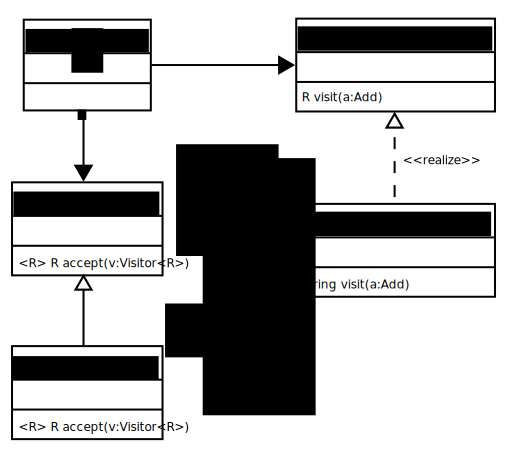
\includegraphics[width=200pt]{VisitorDiagram}
    }
  \end{figure}
\end{slide}


\begin{slide}{Internal visitor pattern}
  \begin{description}
    \item[Internal visitor] Visitor pattern where elements specify control flow.
  \end{description}
  Object Algebra Interface:
  \begin{java}
interface IntAlg<R> {
  R lit(int x);
  R add(R e1, R e2);
}
  \end{java}
The parameter \inlinecode{java}{R} represents the result type.
  Note: explicit mention of constructors means using standard visitor pattern we are unable to add new data variants.
\end{slide}


\begin{slide}{Internal visitor pattern}{Implementation}
  \begin{java}
interface Expr {
  <R> R accept(IntAlg<R> vis);
}
class Add implements Expr {
  Exp left, right;
  public Add(Expr left, Expr right) { 
    this.left = left; 
    this.right = right;
  }
  public <R> R accept(IntAlg<R> vis) {
    return vis.add(left.accept(vis), right.accept(vis));
  }
}
  \end{java}
  Behavious is supplied by the visitor.
  Accept methods apply function from visitor recursively.
\end{slide}


\begin{slide}{Internal visitor pattern}{Implementation}
\begin{java}
class PrintVisitor implements IntAlg<String> {
  public String lit(int x) {
    return new Integer(x).toString();
  }
  public String add(String e1, String e2) {
    return e1 + " + " + e2;
  }
}
\end{java}
\begin{itemize}
\item Code can now be grouped by operation rather than class.
\item Notion of state relative to an operation instead of a class.
\end{itemize}
\end{slide}


\begin{slide}{Visitor pattern analysis}
Unfortunately, we lose the ability to add data variants..
It seems we traded one kind of extensibility for another.

%The problem is that we used a concrete reference to IntAlg in previous data variants.
%To add new data variants, we have to adjust our IntAlg interface which is a violation.
Concrete \inlinecode{java}{IntAlg<R>} reference is the problem:
\begin{java}
interface Expr {
  <R> R accept(IntAlg<R> vis);
}
\end{java}

No accept method $\implies$ No retroactive implementation.
%Classes require accept method -> No retroactive implementation.
\end{slide}


%  Church encoding?
%%%%%%%%%%%%%%%%%%%%%%%%%%%%%%%%%%%%%%%%%%%%%%%%%%%%%%%%%%%%%%%%%%%%%%%%%%%%%%%%%%%%%%%%%%%%%%%%%%%%%%%%%%%%%%%%%%%%%%%
%%%%  Object Algebras
%%%%%%%%%%%%%%%%%%%%%%%%%%%%%%%%%%%%%%%%%%%%%%%%%%%%%%%%%%%%%%%%%%%%%%%%%%%%%%%%%%%%%%%%%%%%%%%%%%%%%%%%%%%%%%%%%%%%%%%
\begin{slide}{Object Algebras}
\begin{description}
\item[Object Algebra] a class that implements a object algebra interface, which corresponds to a particular kind of algebraic signature
\end{description}
\end{slide}


\begin{slide}{Object Algebra}{Example of a Factory}
An Object Algebra representing a Factory.
\begin{java}
class IntFactory implements IntAlg<Expr> {
  public Expr lit(int x) {
    return new Lit(x);
  }
  public Expr add(Expr e1, Expr e2) {
    return new Add(e1, e2);
  }
}
\end{java}
\end{slide}

\begin{slide}{Object Algebras}{Church encoding}
\begin{description}
\item[Church encoding] Representing data and operators in the lambda calculus % named for Alonzo Church who first represented data this way.
\end{description}

Model expressions as church values representing the shape of an expression using the object algebra interface.
We parameterize expressions with object algebras.% such that behaviour is supplied later. 
%This way expressions are parameterized with an object algebra such that desired behaviour can be supplied later.
%The desired behaviour is supplied with object algebras.
An example of a church encoded value:
\begin{java}
<R> R make3Plus5(IntAlg<R> f) {
  return f.add( f.lit(3), f.lit(5) );
}
\end{java}
We then supply the object algebra to the church encoded value:
\begin{java}
Expr e = make3Plus5(new IntFactory());
\end{java}
% Note: You can use parsers to construct church encoded values.
\end{slide}

\begin{slide}{Object Algebras}{Retroactive implementation}
We have seen:
  Visitor pattern is no solution as it requires modification of existing code.

But with church encoded values:
We can add new operations to our data type by introducing new object algebras.
We can add new data variants by extending the object algebra interface, and corresponding object algebras.
\end{slide}


\begin{slide}{Data variant extension}
Let's see how we can extend these object algebras.
We already have:
\begin{java}
interface IntAlg<R> {
  R lit(int x);
  R add(R e1, R e2);
}
\end{java}
We add new data variants to the object algebra interface:
\begin{java}
interface IntBoolAlg<R> extends IntAlg<R> {
  R bool(Boolean b);
  R iff(R e1, R e2, R e3);
}
\end{java}
\end{slide}

\begin{slide}{Extension of factory object algebra}
And finally extend the object algebra:
\begin{java}
class Bool implements Expr {...}
class Iff implements Expr {...}

class IntBoolFactory extends IntFactory 
                     implements IntBoolAlg<Expr> {
  public Expr bool(Boolean b) {
    return new Bool(b);
  }
  public Expr iff(Expr e1, Expr e2, Expr e3) {
    return new Iff(e1,e2,e3);
  }
}
\end{java}
\end{slide}

\begin{slide}{Prettyprinting extension}
An object algebra for pretty printing:
\begin{java}
class IntBoolPrintVisitor extends PrintVisitor 
                          implements IntBoolAlg<string> {
  public string bool(final Boolean b) {
    return new Boolean(b).toString();
  }
  public string iff(final string e1, final string e2, final string e3) {
    return "if (" + e1 + ") then " + e2 + " else " + e3;
  }
}
\end{java}
\end{slide}



\begin{slide}{Synthesized attributes}
So far we have been using operations that are formed from bottom up and do not require additional information.
Object approach vs bottom up approach (bottom up a lot cleaner)
show synthesized attribute and inherited attribute.

Inherited attributes can also be done:
\begin{enumerate}
\item in Java with anonymous classes
\item in C\# with delegates as result type
\end{enumerate}

\begin{java}
interface Printable {
  string pretty();
}

class Implementation implements IntAlg<Printable>
{
  
}

\end{java}
\end{slide}


%misschien goede plek voor inherited attributes.

%%%%%%%%%%%%%%%%%%%%%%%%%%%%%%%%%%%%%%%%%%%%%%%%%%%%%%%%%%%%%%%%%%%%%%%%%%%%%%%%%%%%%%%%%%%%%%%%%%%%%%%%%%%%%%%%%%%%%%%
%%%%  Subtyping relations
%%%%%%%%%%%%%%%%%%%%%%%%%%%%%%%%%%%%%%%%%%%%%%%%%%%%%%%%%%%%%%%%%%%%%%%%%%%%%%%%%%%%%%%%%%%%%%%%%%%%%%%%%%%%%%%%%%%%%%%
\begin{slide}{Subtyping relations}
\begin{itemize}
\item Subtyping between extended and base terms. 
\item Subtyping between operations on those terms.
\end{itemize}
Not many other solutions to the EP support such subtyping relations.
%expression families problem,
\end{slide}

\begin{slide}{Subtyping operations}

We can supply extended object algebras to terms that only rely on some super type.
\inlinecode{java}{string pp = make3Plus5(new IntBoolPrintVisitor());}

This subtyping relation follows from OO's subtyping on interfaces.

The other way around results in a type error:
\inlinecode{java}{string pp = ifTrueThenExpElseConst0(new PrintVisitor());} %todo insert code
as PrintVisitor is unable to supply implementations for \inlinecode{java}{iff} and \inlinecode{java}{bool}.
\end{slide}

\begin{slide}{Subtyping terms}

\begin{java}
<R> R exp(IntAlg<R> v) {
  return v.add(v.lit(3), v.lit(4));
}
\end{java}
\begin{java}
<R> R exp2(IntBoolAlg<R> v) {
  return v.iff(v.bool(false), exp(v), v.lit(0));
}
\end{java}

\end{slide}


%%%%%%%%%%%%%%%%%%%%%%%%%%%%%%%%%%%%%%%%%%%%%%%%%%%%%%%%%%%%%%%%%%%%%%%%%%%%%%%%%%%%%%%%%%%%%%%%%%%%%%%%%%%%%%%%%%%%%%%
%%%%  Multi-sorted object algebras
%%%%%%%%%%%%%%%%%%%%%%%%%%%%%%%%%%%%%%%%%%%%%%%%%%%%%%%%%%%%%%%%%%%%%%%%%%%%%%%%%%%%%%%%%%%%%%%%%%%%%%%%%%%%%%%%%%%%%%%
\begin{slide}{Multi-sorted object algebras}
Evolve multiple recursive types as family.

Lets introduce a new syntactic sort \inlinecode{java}{Statement}:
\begin{java}
interface StmtAlg<R,S> extends IntBoolAlg<R> {
  R var(String x);
  R assign(String x, R e);
  S expr(R e);
  S comp(S s1, S s2);
}
\end{java}
%todo Closely related to family polymorphism.
\end{slide}

\begin{slide}{StmtFactory object algebra}
Use of anonymous inner classes to implement interface. % Not possible in C#  (use delegates instead)
\begin{java}
interface Stmt {
  void eval();
}
class StmtFactory extends IntBoolFactory
                  implements StmtAlg<Expr,Stmt> {
  HashMap<String,int> map = new HashMap<String,int>();
  public Expr var(String x) {
    return new Expr() {
      public int eval() {
        return map.get(x);
      }
    }
  }
  public Expr assign(String x, Expr e) { .. }
  public Stmt comp(Stmt s1, Stmt s2) { .. }
  public Stmt expr(Expr e) { .. }
}
\end{java}
\end{slide}
%%%%%%%%%%%%%%%%%%%%%%%%%%%%%%%%%%%%%%%%%%%%%%%%%%%%%%%%%%%%%%%%%%%%%%%%%%%%%%%%%%%%%%%%%%%%%%%%%%%%%%%%%%%%%%%%%%%%%%%
%%%%  Modular combination of algebras
%%%%%%%%%%%%%%%%%%%%%%%%%%%%%%%%%%%%%%%%%%%%%%%%%%%%%%%%%%%%%%%%%%%%%%%%%%%%%%%%%%%%%%%%%%%%%%%%%%%%%%%%%%%%%%%%%%%%%%%

\begin{slide}{Modular combination of algebras}
Instead of extending \inlinecode{java}{IntAlg<R>}, we define \inlinecode{java}{BoolAlg<R>} seperately.
\begin{java}
interface BoolAlg<R> {
  R bool(boolean x);
  R iff(R b, R e1, R e2);
}
\end{java}
Due to java's multiple interface inheritance we can define:
\inlinecode{java}{interface ExpIntBool<R> extends BoolAlg<R>, IntAlg<R> {}}
\end{slide}

\begin{slide}{Union combinator}
Unfortunately combining object algebras is not as easy.
We have to delegate functions to their implementations:
\begin{java}
class Union<R> implements ExpIntBool<R> {
  BoolAlg<R> v1;
  IntAlg<R> v2;
  Union(BoolAlg<R> v1, IntAlg<R> v2) { this.v1 = v1; this.v2 = v2; }
  public R lit(int x) { return v2.lit(x); }
  public R add(R e1, R e2) { return v2.add(e1, e2); }
  public R bool(Boolean b) { return v1.bool(b); }
  public R iff(R e1, R e2, R e3) { return v1.iff(e1, e2, e3); }
}
\end{java}
\end{slide}
\begin{slide}{Union object algebra}
We can now create modular object algebras by instantiating each object algebra individually:

\begin{java}
class IntBoolFactory2 extends Union<Expr> {
  IntBoolFactory2() { super(new BoolFactory(), new IntFactory()); }
}
\end{java}
\end{slide}

\begin{slide}{Combine combinator}
So far, we only computed one operation (or attribute).
Suppose that now we want to compute multiple operations, they can even be dependent.
\begin{java}
class Pair<A, B> {
  A a; B b;
  Pair(A a, B b) { this.a = a; this.b = b; }
  A a() { return a; }
  B b() { return b; }
}
\end{java}
\end{slide}

\begin{slide}{Combine combinator}
We can now compute multiple operations using the \inlinecode{java}{Combine<A,B>} combinator:
\begin{java}
class Combine<A, B> implements IntAlg<Pair<A, B>> {
  IntAlg<A> v1;
  IntAlg<B> v2;
  Combine(IntAlg<A> v1, IntAlg<B> v2) { this.v1 = v1;this.v2 = v2; }
  public Pair<A, B> lit(int x) {
    return new Pair<A, B>(v1.lit(x), v2.lit(x));
  }
  public Pair<A, B> add(Pair<A, B> e1, Pair<A, B> e2) {
    return new Pair<A, B>(v1.add(e1.a(), e2.a()), v2.add(e1.b(), e2.b()));
  }
}
\end{java} 
\end{slide}
\begin{slide}{About independent extensibility}
We have to reimplement the combinators for extension of the object algebra interface.
However using bounded polymorphism we can ease the burden somewhat:
\begin{java}
class GUnion<R,V1 extends BoolAlg<R>, V2 extends BoolAlg<R>> implements IntBoolAlg<R> {
  ..
}
\end{java}
So now we can extend \inlinecode{java}{GUnion} to allow extensions for the components.
\end{slide}

\begin{slide}{Related Work}
A lot of solutions are not statically type safe or rely on advanced language features.
%TODO:
\end{slide}

\begin{slide}{Conclusion}
New solution to the expression problem:
\begin{itemize}
\item relies only on basic generics (parametric polymorphism)
\item similar to visitor pattern but without accept functions
\item retroactive implementation
\end{itemize}
Language extensions are still useful
for example: automatically provide combinators.
\end{slide}

% Thank you & CREDIT slide


\begin{slide}
Object algebras do not have to rely on advanced programming techniques and can be implemented just relying on basic generics.
  \begin{itemize}
    \item F-bounded quantification
    \item wildcards
    \item variance annotations.
  \end{itemize}
\end{slide}

\begin{slide}{Example OO code}
Like the following:
\begin{java}
interface Exp {
    Value eval();
}
class Lit implements Exp {
    int x;
    public Lit(int x) { this.x = x; }
    public Value eval() {
        return new VInt(x);
}}
class Add implements Exp {
    Exp l, r;
    public Add(Exp l, Exp r) { this.l = l; this.r = r; }
    public Value eval() {
        return new VInt(l.eval().getInt() + r.eval().getInt());
}}
\end{java}
\end{slide}

\section{Elements}

\begin{frame}[fragile]
  \frametitle{Typography}
      \begin{minted}[fontsize=\small]{latex}
The theme provides sensible defaults to \emph{emphasize}
text, \alert{accent} parts or show \textbf{bold} results.
      \end{minted}

  \begin{center}becomes\end{center}
  
\begin{minted}[mathescape,
               linenos,
               numbersep=5pt,
               gobble=2,
               frame=lines,
               framesep=2mm]{csharp}
  string title = "This is a Unicode π in the sky"
  /*
  Defined as $\pi=\lim_{n\to\infty}\frac{P_n}{d}$ where $P$ is the perimeter
  of an $n$-sided regular polygon circumscribing a
  circle of diameter $d$.
  */
  const double pi = 3.1415926535
\end{minted}

  The theme provides sensible defaults to \emph{emphasize} text,
  \alert{accent} parts or show \textbf{bold} results.
\end{frame}
\begin{frame}{Lists}
  \begin{columns}[onlytextwidth]
    \column{0.5\textwidth}
      Items
      \begin{itemize}
        \item Milk \item Eggs \item Potatos
      \end{itemize}

    \column{0.5\textwidth}
      Enumerations
      \begin{enumerate}
        \item First, \item Second and \item Last.
      \end{enumerate}
  \end{columns}
\end{frame}
\begin{frame}{Descriptions}
  \begin{description}
    \item[PowerPoint] Meeh.
    \item[Beamer] Yeeeha.
  \end{description}
\end{frame}
\begin{frame}{Animation}
  \begin{itemize}[<+- | alert@+>]
    \item \alert<4>{This is\only<4>{ really} important}
    \item Now this
    \item And now this
  \end{itemize}
\end{frame}
\begin{frame}{Figures}
  \begin{figure}
    \newcounter{density}
    \setcounter{density}{20}
    \begin{tikzpicture}
      \def\couleur{mLightBrown}
      \path[coordinate] (0,0)  coordinate(A)
                  ++( 90:5cm) coordinate(B)
                  ++(0:5cm) coordinate(C)
                  ++(-90:5cm) coordinate(D);
      \draw[fill=\couleur!\thedensity] (A) -- (B) -- (C) --(D) -- cycle;
      \foreach \x in {1,...,40}{%
          \pgfmathsetcounter{density}{\thedensity+20}
          \setcounter{density}{\thedensity}
          \path[coordinate] coordinate(X) at (A){};
          \path[coordinate] (A) -- (B) coordinate[pos=.10](A)
                              -- (C) coordinate[pos=.10](B)
                              -- (D) coordinate[pos=.10](C)
                              -- (X) coordinate[pos=.10](D);
          \draw[fill=\couleur!\thedensity] (A)--(B)--(C)-- (D) -- cycle;
      }
    \end{tikzpicture}
    \caption{Rotated square from
    \href{http://www.texample.net/tikz/examples/rotated-polygons/}{texample.net}.}
  \end{figure}
\end{frame}
\begin{frame}{Tables}
  \begin{table}
    \caption{Largest cities in the world (source: Wikipedia)}
    \begin{tabular}{lr}
      \toprule
      City & Population\\
      \midrule
      Mexico City & 20,116,842\\
      Shanghai & 19,210,000\\
      Peking & 15,796,450\\
      Istanbul & 14,160,467\\
      \bottomrule
    \end{tabular}
  \end{table}
\end{frame}
\begin{frame}{Blocks}

  \begin{block}{This is a block title}
    This is soothing.
  \end{block}

\end{frame}
\begin{frame}{Math}
  \begin{equation*}
    e = \lim_{n\to \infty} \left(1 + \frac{1}{n}\right)^n
  \end{equation*}
\end{frame}
\begin{frame}{Line plots}
  \begin{figure}
    \begin{tikzpicture}
      \begin{axis}[
        mlineplot,
        width=0.9\textwidth,
        height=6cm,
      ]

        \addplot {sin(deg(x))};
        \addplot+[samples=100] {sin(deg(2*x))};

      \end{axis}
    \end{tikzpicture}
  \end{figure}
\end{frame}
\begin{frame}{Bar charts}
  \begin{figure}
    \begin{tikzpicture}
      \begin{axis}[
        mbarplot,
        xlabel={Foo},
        ylabel={Bar},
        width=0.9\textwidth,
        height=6cm,
      ]

      \addplot plot coordinates {(1, 20) (2, 25) (3, 22.4) (4, 12.4)};
      \addplot plot coordinates {(1, 18) (2, 24) (3, 23.5) (4, 13.2)};
      \addplot plot coordinates {(1, 10) (2, 19) (3, 25) (4, 15.2)};

      \legend{lorem, ipsum, dolor}

      \end{axis}
    \end{tikzpicture}
  \end{figure}
\end{frame}
\begin{frame}{Quotes}
  \begin{quote}
    Veni, Vidi, Vici
  \end{quote}
\end{frame}


\section{Conclusion}

\begin{frame}{Summary}

  Get the source of this theme and the demo presentation from

  \begin{center}\url{github.com/matze/mtheme}\end{center}

  The theme \emph{itself} is licensed under a
  \href{http://creativecommons.org/licenses/by-sa/4.0/}{Creative Commons
  Attribution-ShareAlike 4.0 International License}.

  \begin{center}\ccbysa\end{center}

\end{frame}

\plain{Questions?}
% Possible questions:
% What advanced language features solve the expression problem?
% In Java you have JavaGI where you can let classes implement interfaces even after object are instantiated.
\end{document}
